\documentclass[tikz,border=6pt]{standalone}
\usepackage{pgfplots}
\pgfplotsset{compat=1.18}
\begin{document}
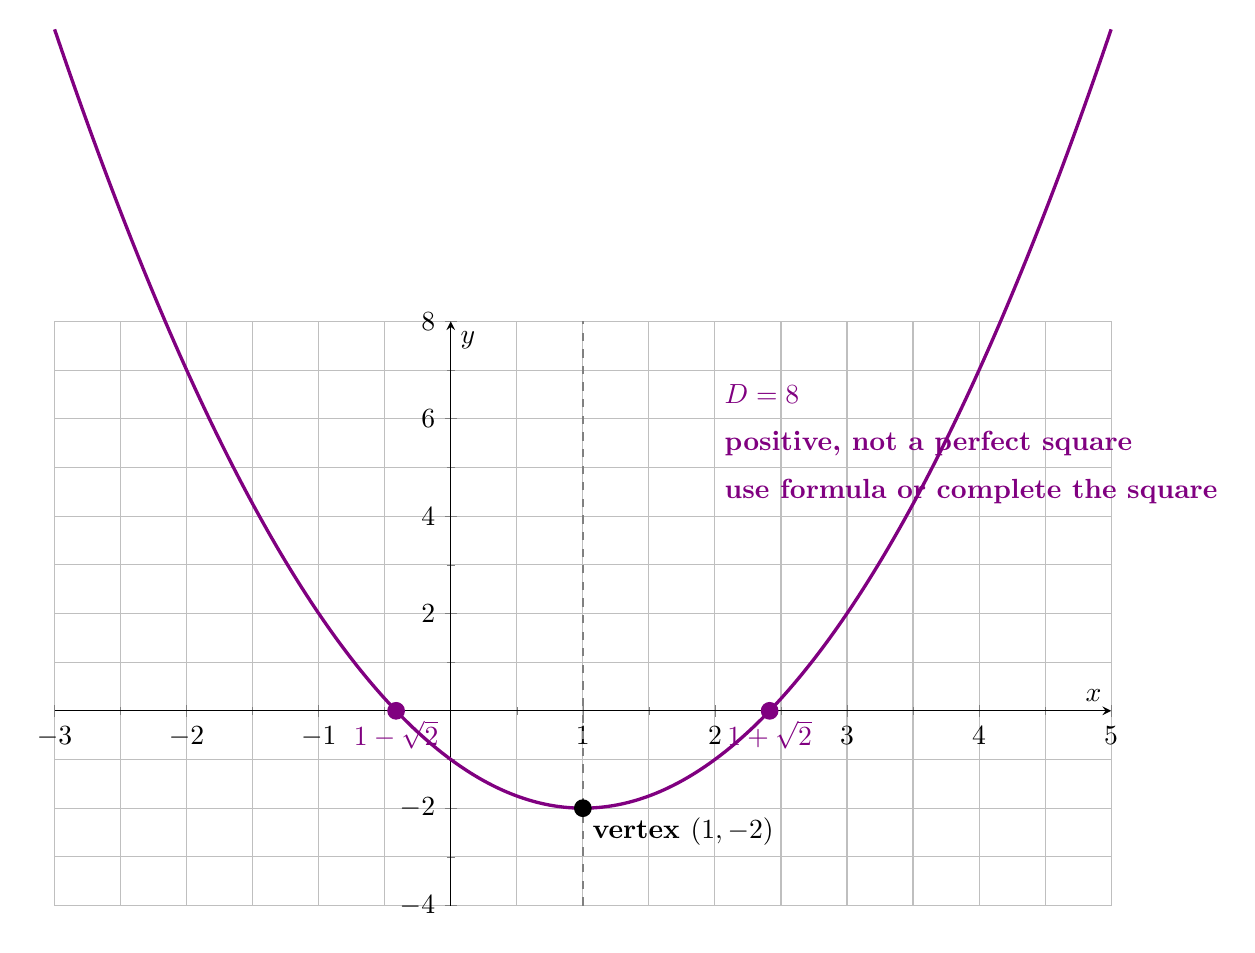
\begin{tikzpicture}
\begin{axis}[
  width=15cm,height=9cm,
  xmin=-3,xmax=5,ymin=-4,ymax=8,
  axis lines=middle,
  xlabel={$x$},ylabel={$y$},
  grid=both,minor tick num=1,
  samples=240,clip=false
]
\addplot[violet,very thick,domain=-3:5]{x^2-2*x-1};
\addplot[gray,dashed,thick] coordinates {(1,-4) (1,8)};
\addplot[violet,only marks,mark=*,mark size=3pt]
  coordinates {({1-sqrt(2)},0) ({1+sqrt(2)},0)};
\addplot[black,only marks,mark=*,mark size=3pt] coordinates {(1,-2)};
\node[violet,font=\bfseries,anchor=north] at (axis cs:{1-sqrt(2)},0) {$1-\sqrt2$};
\node[violet,font=\bfseries,anchor=north] at (axis cs:{1+sqrt(2)},0) {$1+\sqrt2$};
\node[black,font=\bfseries,anchor=north west] at (axis cs:1,-2) {vertex $(1,-2)$};
\node[violet,font=\bfseries,anchor=west] at (axis cs:2.0,6.5) {$D=8$};
\node[violet,font=\bfseries,anchor=west] at (axis cs:2.0,5.5) {positive, not a perfect square};
\node[violet,font=\bfseries,anchor=west] at (axis cs:2.0,4.5) {use formula or complete the square};
\end{axis}
\end{tikzpicture}
\end{document}
